
\documentclass{Setup/template_isec_class}

% Template ISEC/LaTeX, janeiro 2023
%--------------------------------------
\usepackage{Setup/template_isec_package}
%--------------------------------------

%--------------------------------------
% Obs#1
% Onde incluir todos os ficheiros (package)
% e instruções adicionais para este projeto
\usepackage{extras}
%--------------------------------------

\begin{document}

%--------------------------------------
% Obs#2
% Definir qual o título e quais os autores do trabalho
\newcommand{\titulotrabalho}{Título do trabalho}
\newcommand{\autorestrabalho}{Autor ou autores do trabalho}
%--------------------------------------

\pagestyle{empty}

% Capa
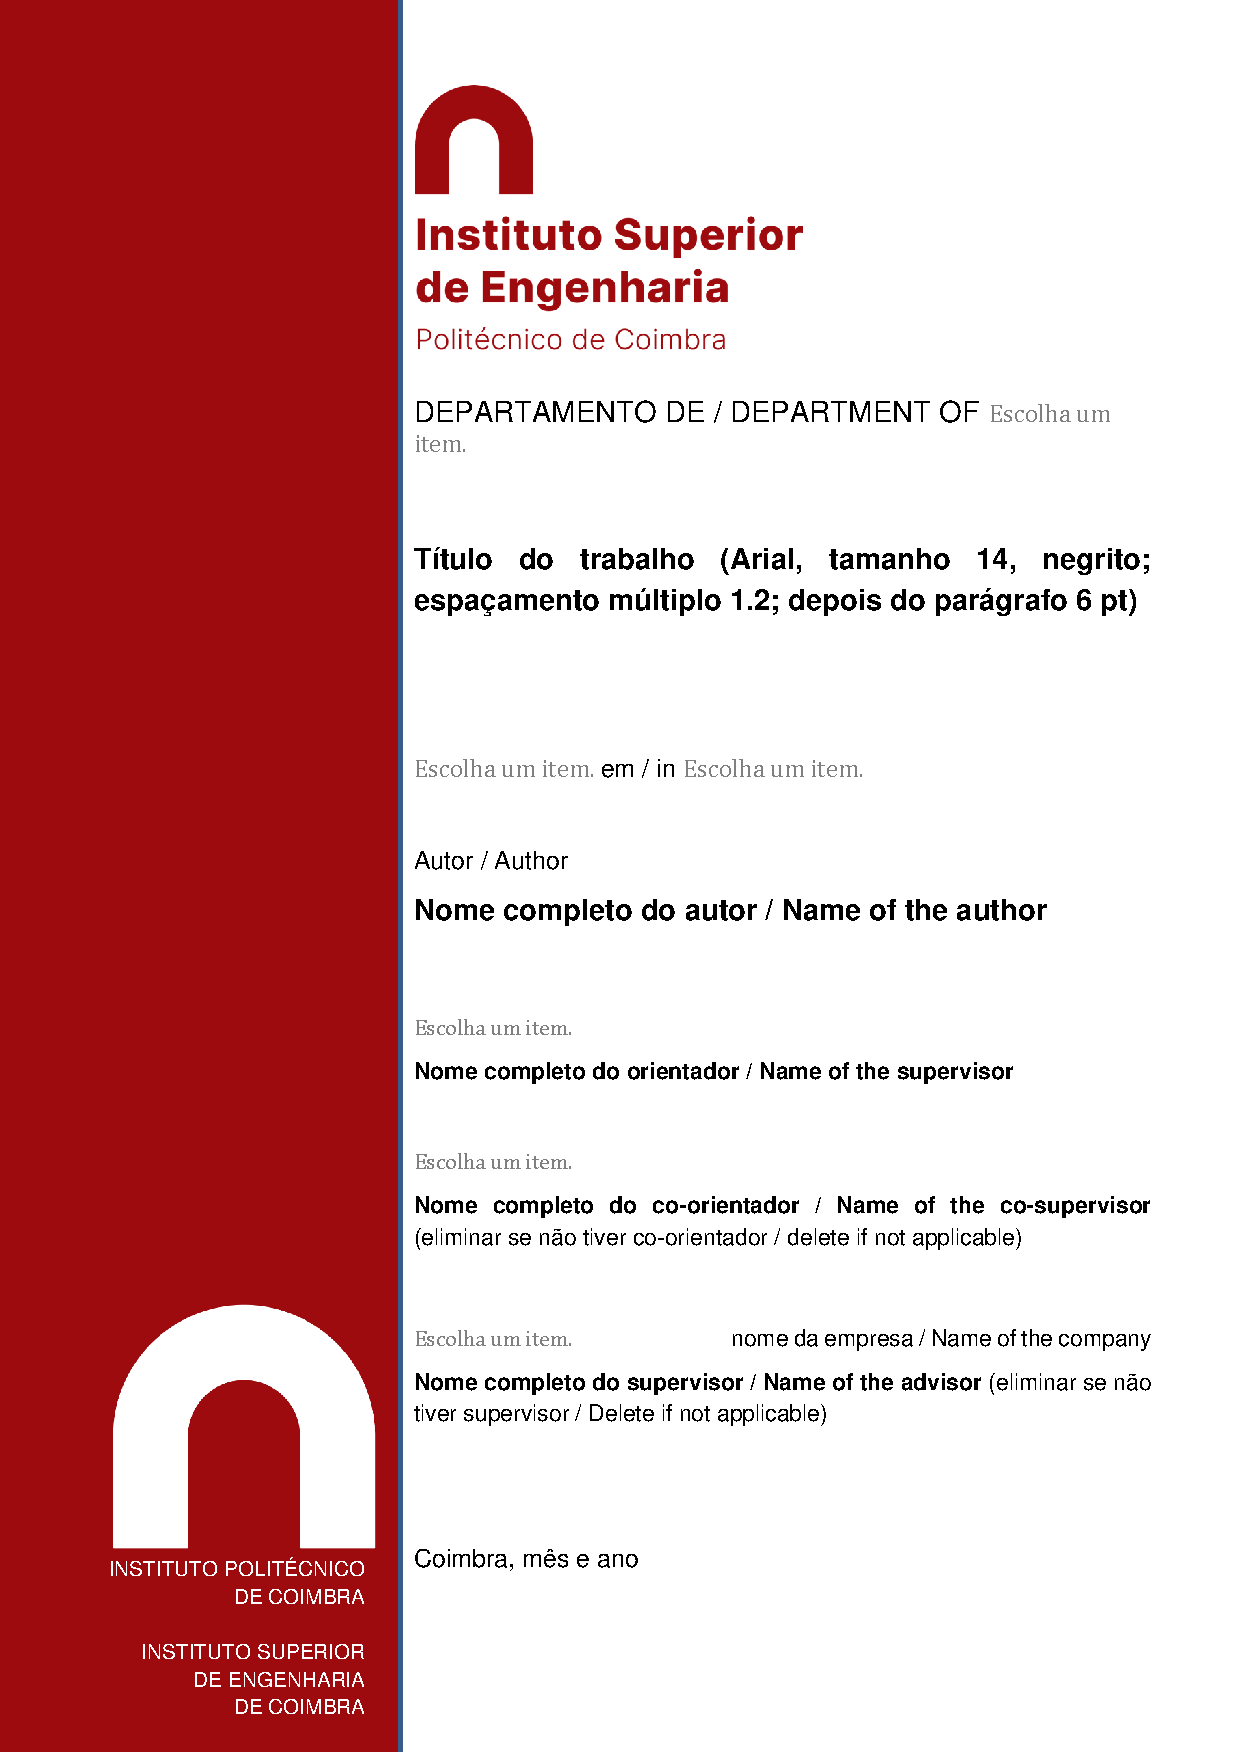
\includepdf{Inicio/capa}

\newpage

%--------------------------------------
\pagestyle{fancy}
\fancyhf{}
\fancyhead{}
\fancyhead[CO]{\nouppercase{\truncate{\headwidth}{\titulotrabalho}}}
\fancyhead[CE]{\nouppercase{\autorestrabalho}}
\renewcommand{\headrulewidth}{0pt}
\fancyfoot{}
\fancyfoot[CO,CE]{\thepage}
\setlength{\headheight}{14.5pt}
\fancypagestyle{plain}{}
%--------------------------------------

\pagenumbering{roman}

% Resumo PT
\phantomsection
\addcontentsline{toc}{chapter}{Resumo}

% Resumo
%--------------------------------------
\vspace*{45pt}
\begin{flushleft}
	{\Large \textbf{\scshape{Resumo}}}
\end{flushleft}
\vspace*{10pt}


%tira a próxima linha e escrever o resumo
\amostradetexto


\vspace*{20pt}

\noindent \textbf{Palavras-chave}:
palavra-chave1, palavra-chave2, palavra-chave3, palavra-chave4.



\newpage

% Abstract ENG
\phantomsection
\addcontentsline{toc}{chapter}{Abstract}

% Abstract
%--------------------------------------
\vspace*{45pt}
\begin{flushleft}
	{\Large \textbf{\scshape{Abstract}}}
\end{flushleft}
\vspace*{10pt}


\amostradetexto


\vspace*{20pt}

\noindent \textbf{Keywords}:
keyword1, keyword2, keyword2, keyword3, keyword4



\newpage

% Epígrafe
\phantomsection
\addcontentsline{toc}{chapter}{Ep\'{\i}grafe}

% Epígrafe
%--------------------------------------
\vspace*{45pt}
\begin{flushleft}
	{\Large \textbf{\scshape{Ep\'{\i}grafe}}}
\end{flushleft}
\vspace*{10pt}

\begin{flushright}
	O começo de todas as ciências é o espanto de as coisas serem o que são. \\
	Aristóteles
\end{flushright}



\newpage

% Dedicatória
\phantomsection
\addcontentsline{toc}{chapter}{Dedicat\'{o}ria}

% Dedicatória
%--------------------------------------
\vspace*{45pt}
\begin{flushleft}
	{\Large \textbf{\scshape{Dedicat\'{o}ria}}}
\end{flushleft}
\vspace*{10pt}


\amostradetexto



\newpage

% Agradecimentos
\phantomsection
\addcontentsline{toc}{chapter}{Agradecimentos}

% Agradecimentos
%--------------------------------------
\vspace*{45pt}
\begin{flushleft}
	{\Large \textbf{\scshape{Agradecimentos}}}
\end{flushleft}
\vspace*{10pt}

Aqui poderá apresentar  os agradecimentos às entidades (p. ex., instituição de ensino, entidade de acolhimento do estágio, etc.) e às pessoas que direta ou indiretamente são merecedoras de tal reconhecimento (família, amigos, professores, etc.).

\newpage

\pagenumbering{arabic}

\renewcommand{\contentsname}{\'{I}ndice}
\renewcommand{\listtablename}{\'{I}ndice de tabelas}
\renewcommand{\listfigurename}{\'{I}ndice de figuras}

\phantomsection
\addcontentsline{toc}{chapter}{\'{I}ndice}
\tableofcontents

\newpage

\phantomsection
\addcontentsline{toc}{chapter}{\'{I}ndice de tabelas}
\listoftables

\newpage

\phantomsection
\addcontentsline{toc}{chapter}{\'{I}ndice de figuras}
\listoffigures

\newpage

% Lista de abreviaturas
\phantomsection
\addcontentsline{toc}{chapter}{Lista de abreviaturas}

% Lista de abreviaturas
%--------------------------------------
\vspace*{45pt}
\begin{flushleft}
	{\Large \textbf{\scshape{Lista de abreviaturas}}}
\end{flushleft}
\vspace*{20pt}

\begin{tabular}{l l}
    IEEE	&  \textit{Institute of Electrical and Electronics Engineers}\\
    ISEC    &  Instituto Superior de Engenharia de Coimbra\\
    % deve acrescentar aqui as abreviaturas que considerar necessárias, por ordem alfabética    
\end{tabular}



\newpage

% Lista de siglas e acrónimos
\phantomsection
\addcontentsline{toc}{chapter}{Lista de siglas e acr\'{o}nimos}

% Lista de siglas e acrónimos
%--------------------------------------
\vspace*{45pt}
\begin{flushleft}
	{\Large \textbf{\scshape{Lista de siglas e acrónimos}}}
\end{flushleft}
\vspace*{20pt}

\begin{tabular}{l l}
    CD      &  \textit{Compact Disc}\\
    ONU     &   Organização das Nações Unidas\\
    % deve acrescentar aqui as siglas e os acrónimos que considerar necessários, por ordem alfabética    
\end{tabular}



\newpage

% Lista de símbolos
\phantomsection
\addcontentsline{toc}{chapter}{Lista de s\'{\i}mbolos}

% Lista de símbolos
%--------------------------------------
\vspace*{45pt}
\begin{flushleft}
	{\Large \textbf{\scshape{Lista de símbolos}}}
\end{flushleft}
\vspace*{20pt}

\begin{tabular}{l l}
    $\mathrm{kN}$       &   Quilonewton\\
    $\varepsilon_{ax}$  &   Extensão axial (\%)\\
    % deve acrescentar aqui os símbolos que considerar necessários, por ordem alfabética    
\end{tabular}



\newpage

% Capítulo inicial
% Introdução

% Introdução
%--------------------------------------
\chapter{Introdução}

O capítulo introdutório deverá ser apresentado neste ficheiro com toda a informação necessária à compreensão do tema/assunto do trabalho. 

Deverão constar os conceitos fundamentais relacionados com o tema do  trabalho, devendo terminar com a descrição genérica da organização do documento.

No que segue é apresentada a forma de importar o \textit{template} para o programa \textit{Overleaf} e como é constituído o próprio \textit{template}  em \LaTeX~ sugerido aos alunos. Para além disso, também se explica como criar e juntar a capa do trabalho ao documento.

Os ficheiros do \textit{template} estão disponíveis na pasta Template4LaTeX4ISEC que está disponível no \textit{site} do ISEC -> serviços académicos $\rightarrow$ formulários $\rightarrow$ licenciatura $\rightarrow$ Template para trabalhos de Licenciatura, Projetos e Relatórios de Estágio $\rightarrow$ ... \\
Dentro desta pasta encontram-se dois ficheiros ZIP relativos a dois projetos. Um dos projetos é o \textit{template} (projeto limpo, apenas com o esqueleto de base) e o outro é um  exemplo que corresponde a um projeto customizado com um nome diferente e com exemplos incluídos. Nessa pasta encontram-se ainda dois ficheiros PDF, em que cada um corresponde à versão impressa de cada um dos projetos supra mencionados.

\section{Como importar o \textit{template} para o Overleaf}
    Nesta secção explicam-se os passos que devem ser seguidos para usar este \textit{template}:
    \begin{enumerate}
        \item Criar conta no Overleaf;
        \item No Overleaf, escolher \textbf{New Project} $\rightarrow$ \textbf{Upload Project} $\rightarrow$ escolher o projeto de nome \textbf{ISEC LaTeX template} previamente guardado em disco tal como ilustra a  Figura~\ref{fig-upload}.
        \item Para fazer o \textit{rename} do projeto, deve selecionar o projeto e proceder como ilustra a Figura~\ref{fig-rename}.% ilustra os passos enunciados anteriormente.
    \end{enumerate}
    
    \begin{figure}[htp]
    	\centering
    	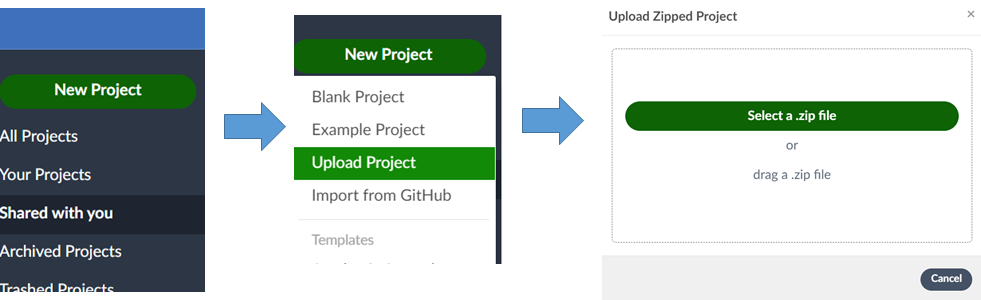
\includegraphics[width=0.8\textwidth]{Figuras/UploadProject}
     \caption{\small{Passos para criar um projeto com base no projeto \textit{template}}}
    	\label{fig-upload}
    \end{figure}

     \begin{figure}[htp]
    	\centering
    	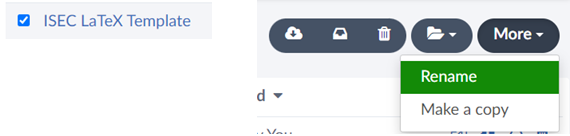
\includegraphics[width=0.6\textwidth]{Figuras/RenameProject}
     \caption{\small{Passos para fazer o \textit{rename} de um projeto}}
    	\label{fig-rename}
    \end{figure}
    
\section{Constituição do \textit{template}}
    
    O \textit{template} é constituído por 5 pastas e 3 ficheiros, cujo teor se descreve de seguida:
    
    \begin{itemize}
        \item Ficheiro \textbf{main.tex}: possui o esqueleto do documento. \textbf{Apenas} deve editar este ficheiro para: 
            \begin{itemize}
                  \item definir o título do trabalho e o nome do autor (procurar por Obs\#2);
                  \item acrescentar ou retirar elementos da estrutura do trabalho como, por exemplo, capítulos ou anexos;
                  \item escolher a formatação das referências bibliográficas: IEEE ou APA (procurar por Obs\#3);
                  \item definir o nome dos anexos (procurar por Obs\#4 e Obs\#5).  
            \end{itemize}
        
        \item Ficheiro \textbf{extras.sty}: na elaboração do documento pode revelar-se necessário a utilização de instruções ou ficheiros adicionais (p. ex., packages, comandos, etc.) devendo os mesmos ser inseridos neste ficheiro; Por exemplo, nas linhas 13, 14 e 15 do ficheiro \verb|extras.sty| estão incluídas as instruções necessárias que ativam as funcionalidades de hipertexto, links e endereços web.
         
        \item Ficheiro \textbf{bibliografia.bib}: é aqui que devem ser colocados os registos de cada uma das referências bibliográficas; neste ficheiro exemplo encontram um  registo de cada um dos possíveis tipos de referências bibliográficas;
        
        \item Pasta \textbf{Setup}: nesta pasta estão incluídos alguns ficheiros específicos do \textit{template}; não pode ser modificada pelo utilizador, sob pena de alterar as características do \textit{template};
    
        \item Pasta \textbf{Início}: todos os ficheiros iniciais do relatório (automaticamente numerados com numeração romana no texto), com extensão *.tex, estão contidos nesta pasta; todos eles devem ser editados com exceção do ficheiro \verb|capa.pdf| e 
        do ficheiro \verb|capa.docx| (ficheiro que apenas se encontra na pasta do projeto gravado localmente no disco). Estes dois ficheiros dizem respeito à criação da capa e são abordados na secção seguinte;
        
        \item Pasta \textbf{Figuras}: é nesta pasta que devem ser colocadas as figuras do documento. Devem ter extensão *.png. Para carregar uma figura para dentro desta pasta devem fazer \textit{Upload} (comando seta no lado esquerdo superior) $\rightarrow$ arrastar a figura para dentro da caixa destino;
    
        \item Pasta \textbf{Capítulos}: dentro desta pasta é onde devem ser colocados os ficheiros *.tex relativos a cada capítulo. Considera-se que o primeiro capítulo é a introdução do trabalho e que o último capítulo é a conclusão do trabalho. Para criar um novo ficheiro *.tex deverá escolher o comando \textit{New File} (comando no lado esquerdo superior);
    
        \item Pasta \textbf{Anexos}: é nesta pasta que devem estar localizados os anexos. Para criar o ficheiro *.tex para um novo anexo, deve proceder de forma idêntica à criação de um novo capítulo.
        
    \end{itemize}
    
    Pode criar novas pastas com o comando \textit{New Folder} (comando no lado esquerdo superior).

\section{Criação da capa do trabalho}

    Para criar a capa do trabalho, deve extrair o conteúdo do ficheiro ZIP associado ao \textit{template}. Deve procurar o ficheiro 
    \verb|capa.docx|, que está dentro da pasta \textbf{Inicio} e customizá-lo. Depois, deve gerar o correspondente ficheiro em formato PDF \verb|capa.pdf| e efetuar o \textit{Upload} desse ficheiro para dentro da pasta \textbf{Inicio} do projeto no Overleaf.
    
\section{Estrutura do documento}
    No Capítulo \ref{cap2} são apresentados alguns exemplos de escrita em \LaTeX, onde são, por exemplo, apresentadas fórmulas matemáticas, tabelas, imagens e muito mais.
    
    No tocante às referências bibliográficas e à escolha do respetivo estilo, deve ser consultado o Capítulo \ref{cap3}.
    
    O trabalho termina com o Capítulo \ref{conclusao} onde são apresentadas as conclusões.

% Capítulo 2

% Segundo capítulo deste trabalho.
%--------------------------------------
\chapter{Título do segundo capítulo}

Esta é a minha primeira referência~\cite{cap2:prf} em \LaTeX.

\amostradetexto



% Capítulo 3

% Terceiro capítulo deste trabalho.
%--------------------------------------
\chapter{Citações e estilos de referências}
\label{cap3}

Este é o terceiro capítulo deste trabalho. 
Na Secção \ref{cap3:citacoes} é indicado como citar uma referência bibliográfica. Os estilos a adotar para as referências bibliográficas são descritos na Secção \ref{cap3:estilosRef}.

\section{Citações}
\label{cap3:citacoes}
    
    Para citar no texto um trabalho previamente incluído nas referências bibliográficas, deve apenas usar-se o comando \verb|\cite| e o respetivo identificador associado a cada uma das referências. 
    
    \subsection{Alguns exemplos}
    
    Aqui pode encontrar exemplos de citações de um artigo \cite{Cohen:1963}, de um livro \cite{CitekeyBook}, de uma secção de um livro \cite{CitekeyInbook}, de um artigo publicado nas atas de um evento \cite{CitekeyInproceedings}, de uns \textit{proceedings} \cite{CitekeyProceedings}, de um manual \cite{CitekeyManual}, de uma tese de mestrado \cite{CitekeyMastersthesis}, de uma tese de doutoramento \cite{CitekeyPhdthesis}, de um relatório técnico \cite{CitekeyTechreport}  
    e de uma referência que não se insere nas categorias anteriores \cite{CitekeyMisc}.
    Se for necessário citar mais do que um trabalho no mesmo ponto do texto, basta separar os trabalhos por vírgulas dentro do comando \verb|\cite|. A título de exemplo, podem citar-se três trabalhos em simultâneo da seguinte forma \cite{Cohen:1963, CitekeyBook,CitekeyInbook}.

\section{Estilo a adotar para as referências bibliográficas}
    \label{cap3:estilosRef}
    
    Os alunos podem escolher utilizar o estilo IEEE ou o estilo APA.
    
    \subsection{Estilo APA}
    \label{cap3:estiloAPA}
    
    Para escolher o estilo APA, deve aceder ao ficheiro \verb+extras.sty+ e procurar por Obs\#1 e descomentar a linha relativa à instrução \verb+\usepackage{apacite}+. \\
    Adicionalmente, no ficheiro \verb+main.tex+ deve procurar a Obs\#3 e descomentar a instrução \verb+\bibliographystyle{apacite}+ e comentar \verb+\bibliographystyle{IEEEtran}+.
    
    \subsection{Estilo IEEE}
    Para escolher o estilo IEEE, deve fazer o procedimento inverso ao descrito na Subsecção \ref{cap3:estiloAPA}, ou seja, deve comentar a instrução \verb+\usepackage{apacite}+ no ficheiro \verb+extras.sty+ (procurar por Obs\#1) bem como comentar a linha \verb+\bibliographystyle{apacite}+ e descomentar a linha \verb+\bibliographystyle{IEEEtran}+ no ficheiro \verb+main.tex+ (procurar por Obs\#3). 
    
    
    

% Capítulo final
% Conclusão

% Conclusão
%--------------------------------------
\chapter{Conclusão}
\label{conclusao}

Aqui devem ser escritas as conclusões do trabalho e, eventualmente, serem apresentadas propostas para trabalho futuro.







\newpage

% Referências bibliográficas
\phantomsection
\addcontentsline{toc}{chapter}{Refer\^{e}ncias bibliogr\'{a}ficas}
\renewcommand{\bibname}{Refer\^{e}ncias bibliogr\'{a}ficas}

%-------------------
% Obs#3
% Descomentar uma das seguintes linhas, em alternativa, 
% consoante o estilo pretendido para as referências bibliográficas
\bibliographystyle{IEEEtran} % formatação segundo IEEE 
%\bibliographystyle{apacite} % formatação segundo APA 
%-------------------
\bibliography{bibliografia}

\newpage

% Anexos
\phantomsection
\addcontentsline{toc}{chapter}{Anexos}
\chapter*{Anexos}

\newpage

% Anexo A
%--------------------------------------
% Obs#4
% Definir o título do anexo A
\newcommand{\tituloanexoA}{Título do Anexo A}
%--------------------------------------
\phantomsection
\addcontentsline{toc}{section}{Anexo A - \tituloanexoA}

% Anexo
%--------------------------------------
\vspace*{45pt}
% Título do anexo A (\tituloanexoA) definido no ficheiro main
\section*{Anexo A - \tituloanexoA}


\amostradetexto



\newpage

% Anexo B
%--------------------------------------
% Obs#5
% Definir o título do anexo B
\newcommand{\tituloanexoB}{Título do Anexo B}
%--------------------------------------
\phantomsection
\addcontentsline{toc}{section}{Anexo B - \tituloanexoB}

% Anexo
%--------------------------------------
\vspace*{45pt}
% Título do anexo B (\tituloanexoB) definido no ficheiro main
\section*{Anexo B - \tituloanexoB}


\amostradetexto



\newpage

\thispagestyle{empty}

% Última página

% Última página
%--------------------------------------

\pagecolor{IsecVermelho}

\mbox{}

\vfill

\begin{center}

\includegraphics[scale=0.3]{Setup/isec-logo}
\end{center}

\newpage

\pagecolor{white}



\end{document}

